\documentclass[11pt]{article}
\usepackage{setspace}
\usepackage{pxfonts}
\usepackage{graphicx}
\usepackage{geometry}

\geometry{letterpaper,left=.5in,right=.5in,top=1in,bottom=.75in,headsep=5pt,footskip=20pt}

\title{Lecture 5 -- Extensions of the Hodgkin-Huxley model}
\author{Computational Neuroscience Summer Program}
\date{June, 2011}

\begin{document}
\maketitle

\paragraph{Motivation.}  The Hodgkin-Huxley model gave us a way to explicitly model ionic currents using the expected conductances of each ion and the driving forces on those ions.  We will now go one step further by explicitly simulating the stochastic actions of individual subunits of the potassium and sodium ion channels.

\paragraph{Potassium channel review.}  The potassium channel is comprised of four identical subunits.  In the Hodgkin-Huxley model, the probability that a given channel is open is equal to $p_K = n^4$, where $n$ is the probability of a single subunit being open.  Recall that $n$ increases when the cell is depolarized and decreases when the cell is hyperpolarized.  The opening rate of each subunit is $\alpha_n$ and the closing rate is $\beta_n$:

\[
\alpha_n(V) = \frac{0.01(V + 55)}{1 - e^{-0.1(V+55)}}
\]

\[
\beta_n(V) = 0.125e^{-0.0125(V+65)}
\]

\paragraph{Stochastic model.}  In the stochastic model, we represent each potassium channel using a state diagram:

\begin{figure}[h]
\begin{center}
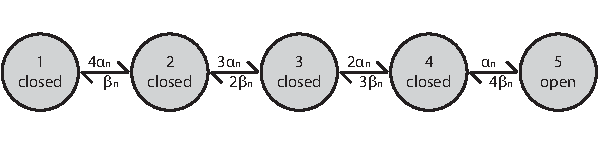
\includegraphics[width=0.75\textwidth]{hodgkin_huxley_advanced/K_state_diagram}
\end{center}
\end{figure}
where the labels represent the probability of transitioning between
each state in the indicated direction.  We simulate a state transition
from state $X$ to $Y$ during a time interval $dt$ if a random number,
chosen with each new timestep of the simulation, is less than the
probability of transitioning between $X$ and $Y$.  The channel is
considered to be open at time $t$ if the ion channel is in the
5$^{th}$ state at time $t$.  In simulations, we'll need to keep track
of how many of the ion channels are open vs. closed during each time
step.  As the number of channels ($N$) increases, this model becomes
arbitrarily similar to the Hodgkin-Huxley version (you'll be verifying
this in the problem set).  Note that you can compute $P_K$ for the
stochastic model at time $t$ by simply computing the fraction of
channels that are in state 5 at time $t$.

\paragraph{Sodium channel review.}  The sodium channel is comprised of three identical subunits and an inactivation gate.  The three identical subunits each open with probability $m$ (where $m$ increases as the cell is depolarized and decreases as the cell is hyperpolarized).  The opening rates for the three subunits are $\alpha_m$, and the closing rates are $\beta_m$.  The inactivation gate is open with probability $h$, where $h$ decreases as the cell is depolarized and increases when the cell is hyperpolarized.  The opening and closing rates are $\alpha_h$ and $\beta_h$, respectively.

\[
\alpha_m(V) = \frac{0.1(V+40)}{1 - e^{-.1(V+40)}}
\]
\[
\beta_m(V) = 4e^{-0.0556(V + 65)}
\]


\[
\alpha_h(V) = 0.07e^{-.05(V+65)}
\]
\[
\beta_n(V) = \frac{1}{1 + e^{-.1(V+35)}}
\]

\paragraph{Stochastic sodium channel model.}  In the Hodgkin-Huxley model, the three subunits and the inactivation gate are assumed to be independent (that's why the probabilities are multiplied into $m^3h$).  However, this is not quite true.  A more accurate description is something like the following:

\begin{figure}[h]
\begin{center}
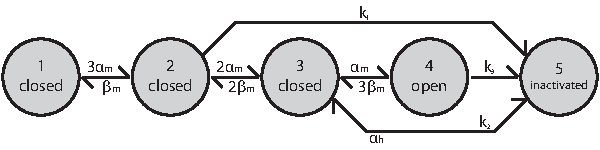
\includegraphics[width=0.75\textwidth]{hodgkin_huxley_advanced/Na_state_diagram}
\end{center}
\end{figure}

In particular, the ball mechanism of the inactivation gate is located inside the cell membrane, and cannot be directly affected by potential across the membrane.  The inactivation gate only comes into play when at least one of the subunits is open (i.e., when the channel occupies states 2, 3, or 4 in the diagram).  In addition, according to this model, if the neuron is in the inactivate state (state 5), it can only transition to state 3.

Whereas the transitions of the three subunits between states 1, 2, 3, and 4 in the stochastic model are identical to in the Hodgkin-Huxley model, the behavior of the inactivation gate is much different -- in particular, the inactivation gate in the stochastic model depends on the states of the three subunits.

As in the stochastic potassium channel model, you can compute the
$P_{Na}$ for the stochastic sodium channel at time $t$ by computing
the fraction of sodium channels which occupy state 4 at that time.

\paragraph{Replacing the Hodgkin-Huxley channels with stochastic
  channels.}  In the Hodgkin-Huxley model, we computed $P_K = n^4$ and
$P_{Na} = m^3h$ with each time step, updating $n, m,$ and $h$ as we
stepped through the model.  In the stochastic model, we compute $P_K$
and $P_{Na}$ directly, so we no longer need to compute $n$, $m$, or
$h$.  Other than the difference in computing $P_K$ and $P_{Na}$, the
stochastic model is identical to the Hodgkin-Huxley model.

\paragraph{Some implementation suggestions.}  There are a number of
possible ways to implement the stochastic channel models, with some
methods being more efficient than others.  Particularly when the
number of channels is large, it becomes very important to code the
simulation efficiently (read: vectorize!) if the simulation is to
finish running in a reasonable amount of time.  To start you off,
we'll go through a simple two-state example.  The states are $x$
(closed) and $y$ (open).  Let's suppose that the probability of
transitioning from state $x$ to state $y$ is $p_{xy}$ and the
probability of transisitioning from $y$ to $x$ is $p_{yx}$.  To
simulate $N = 1000$ of these simple two-state channels, we could write
something like the following:
\newpage
\begin{verbatim}
dt = 0.1;
t = 0:dt:1000;
states = ones(1,N);
n_open = zeros(size(t));

pOpen = [p_xy 0];
pClose = [0 p_yx];
for i = 1:length(t)
  open_chooser = rand(size(states)) < (dt*pOpen(states));
  states(open_chooser) = states(open_chooser) + 1;
  
  close_chooser = rand(size(states)) < (dt*pClose(states));
  states(close_chooser) = states(close_chooser) - 1;
  
  n_open(i) = sum(states == 2);
end
\end{verbatim}

The potasium channel simulation is identical to the above code, but
with the \texttt{pOpen} and \texttt{pClose} variables modified as in
the state diagram.  To implement the stochastic sodium channel model,
you need to seperately compute the probabilities of opening subunits and opening the inactivation gate.

\end{document}


